\documentclass[10pt,conference,compsocconf]{IEEEtran}

%\usepackage{times}
%\usepackage{balance}
\usepackage{url, amsmath, amssymb}
\usepackage{graphicx}    % For figure environment
\usepackage{textcomp}
\usepackage{amsfonts}
\usepackage[ruled,vlined]{algorithm2e}
\SetKwComment{Comment}{$\triangleright$\ }{}

\usepackage[hidelinks,bookmarksnumbered,unicode]{hyperref} % Enables cross linking in the electronic document version. This package has to be included second to last.
\usepackage[noabbrev,nameinlink]{cleveref}
\usepackage{balance}
\usepackage{nag}       % Issues warnings when best practices in writing LaTeX documents are violated.
\usepackage{booktabs}
\usepackage{amsmath}   % Improves the typesettings of tables.

%\DeclareMathOperator*{\argmin}{\arg\!\min}
\DeclareMathOperator*{\argmin}{argmin}   % Jan Hlavacek

\newcommand{\spacing}{\hspace{1cm}}

\usepackage{xcolor}
\newcommand{\todo}[1]{\textcolor{red}{#1}}
%\newcommand{\todo}[1]{{\color{red}{#1}}}

\usepackage{float}

\begin{document}
    \setlength{\abovedisplayskip}{2pt}
    \setlength{\belowdisplayskip}{2pt}
    \setlength{\abovedisplayshortskip}{2pt}
    \setlength{\belowdisplayshortskip}{2pt}
    \title{On Bayesian Factorization Machines in Collaborative Filtering}

    \author{
        Rafael Sterzinger \spacing Patrik Okanovic \spacing Fatjon Zogaj \spacing Filip Batur Stipic\\
        Group: Terminators\\
        Department of Computer Science, ETH Zurich, Switzerland
    }

    \maketitle

    \begin{abstract}
        Collaborative filtering methods for recommender systems find their application in a wide variety of areas.
        In this work we consider several neural-based and standard matrix-factorization-based models, placing our focus on Bayesian Factorization Machines.
        We extended these by adding additional features such as implicit user/item information, multiple user similarity measures, item distance metrics, as well as unsupervised-learned clusters and report results in an extensive benchmark.
    \end{abstract}


    \section{Introduction}

    The goal of recommender systems is to design a model which is capable of estimating a user's preference on some kind of items, in our case movies.
    This is usually done by means of collaborative filtering, a standard computational method that attempts to solve this problem by leveraging similarities between users and items based on previously collected data~\cite{CF_survey}.
    This data usually consists of user/item pairs and its corresponding rating which is normally presented in form of a real-valued sparse matrix.
    This sparseness stems from the majority of user/item pairs being unavailable.

    In this project we are concerned with completing such a sparse matrix in the setting of movie recommendation systems, a problem for which benchmarks such as the Netflix Prize~\cite{Netflix} and the different versions of MovieLens~\cite{Movielens} are already well-established.

    We view these benchmarks as guidelines to select 7 state-of-the-art models allowing for a rigorous evaluation of our final results.
%    We selected standard techniques, mainly based on matrix factorization.
    These include Singular Value Decomposition~\cite{svd}, Non-Negative Matrix Factorization~\cite{6165290}, and variants of Bayesian Factorization Machines~\cite{freudenthaler_bayesian_2011, salakhutdinov_bayesian_2008}.
    As an alternative, we explored different, more recent neural-based methods such as Neural Collaborative Filtering~\cite{DBLP:journals/corr/abs-1708-05031}, autoencoders~\cite{inproceedings} and other autoencoder-like networks.
    Here, we selected the KernelNet~\cite{pmlr-v80-muller18a}, and the AutoRec model~\cite{inproceedings}.


    \section{Models and Methods}
%    In the following section we provide a brief overview of our selected baselines, which served as a starting point for exploring the field of collaborative filtering.

    \subsubsection{Preprocessing | Missing Values Initialization}\label{subsub:missing_init}
    As the majority of our models depends on the whole data matrix as input, we experiment with a variety of initialization techniques for the unobserved values.
    Our approaches include replacement by the total mean, user mean and item mean of rankings.
    We add upon this by enabling models to be used for predicting the unobserved values for others which additionally allows us to iteratively chain multiple models.

    \subsubsection{Postprocessing | Clipping/Rounding}
    As a final step, after prediction, we try various ways of postprocessing the output.
    Among those, is the default way of simply clipping the rating between 1 and 5, rounding to the nearest integer as well as to the nearest quarter.
    We based this idea on the fact that ratings are given as integers and as such errors might be avoidable if the prediction is rounded.

    \subsection{Matrix-Factorization-based Approaches}

    \subsubsection{Singular Value Decomposition \textbf{(SVD)}}

    SVD is a matrix factorization technique that decomposes the original matrix $\mathbf{A} \in {\rm I\!R}^{n \times m} $ into the form $ \mathbf{A} = \mathbf{U \Sigma V}^T $ where $\mathbf{U} \in {\rm I\!R}^{n \times n}$,  $\mathbf{V}  \in {\rm I\!R}^{m \times m}$ are orthogonal matrices and $\mathbf{\Sigma} \in {\rm I\!R}^{n \times m}$ is a diagonal matrix of singular values~\cite{svd}.

    Since the matrix in our setting is sparse, we initialize the missing values as mentioned in \Cref{subsub:missing_init} to be able to apply SVD.
    Afterwards, we select only a subset of the largest $k$ singular values and its associated feature vectors in order to obtain a more generalized low-rank approximation.
    This approximation is guaranteed to obtain the best low-rank approximation of the initial matrix $\mathbf{A}\approx \mathbf{U}_k \mathbf{\Sigma}_k \mathbf{V}^T_k$~\cite{Eckart1936}.

    \subsubsection{Non-Negative Matrix Factorization \textbf{(NMF)}}

    Since the ratings in the matrix are non-negative, another feasible approach is to consider NMF which decomposes our original matrix into $\mathbf{A} = \mathbf{UV}$, where $\mathbf{U}$ and $\mathbf{V}$ are both non-negative~\cite{gillis2014nonnegative}.
    It optimizes over the Frobenius norm between the difference of the observed entries of the approximation and the original matrix, i.e. $ \frac{1}{2}\|\mathbf{\Pi}_{\Omega}(\mathbf{A} - \mathbf{UV})\|^2_F$, in combination with Alternating Least Squares~\cite{als}.
%    NMF leverages the separability of latent parameters %that depend on $\mathbf{U}$ and $\mathbf{V}$ respectively, for example
%    by using Alternating Least Squares~\cite{als}.

    \subsubsection{Bayesian Factorization Machines \textbf{(BFM)}}
    For our last matrix-factorization-based approach, we explored BFM which are Bayesian variants of the former known Factorization Machines \textbf{(FM)}~\cite{rendle_factorization_2010}.
    In its core, FMs build upon the advantages of Support Vector Machines \textbf{(SVM)}but use a factorized parametrization instead of a dense one.
    With this parametrization, FMs are able to estimate all possible interactions between entries even in setting where the data matrix $\mathbf{X}$ is highly sparse.
    Similarly to SVMs with a polynomial kernel, the FM model equation which captures all single and pairwise interactions, can be formulated as:
    $$\hat{y}(\mathbf{x})=w_0+\sum^n_{i=1}w_ix_i + \sum^n_{i=1}\sum^n_{j=i+1}\langle \mathbf{v}_i,\mathbf{v}_j \rangle x_ix_j$$
    Here, $\mathbf{v}_i$ denotes a vector in $\mathbb{R}^k$ which describes the $i$-th variable with $k$ dimensions and $\langle \mathbf{v_i},\mathbf{v_j} \rangle$ the interaction between the variables $i$ and $j$.
    Instead of using a fixed weight $w_{ij}$, this factorization via the dot product allows FMs to predict parameters for related interaction, e.g. different users but same movie.
    In the non-Bayesian setting, model parameters are optimized with stochastic gradient descent.
    As opposed to this, model parameters of Bayesian variants of FMs are optimized via maximum a posteriori estimation by means of Markov Chain Monte Carlo methods for approximate inference~\cite{salakhutdinov_bayesian_2008}.
    This Bayesian approach does not only increase accuracy but also omits the need of exhaustive parameter tuning~\cite{freudenthaler_bayesian_2011}.
    Regarding the implementation of our baseline, we utilize a package named \textit{myFM}~\cite{noauthor_myfm_nodate} which employs Gibbs sampling for approximate inference of the posterior.
    Multiple additions have been made by means of exploiting additional implicit information about users, items, and temporal dynamics~\cite{rendle_scaling_2013,koren_factorization_2008,koren_collaborative_2009}.
    Two implicit features we add are defined as follows:
    \begin{enumerate}
        \item Implicit User Feature \textbf{(Bayesian SVD++)} \\ $\Leftrightarrow$ all items rated by user $u$:
        $$\mathbf{V}_u=\frac{\mathbf{\Omega}_u}{\sqrt{|\{(u,i): (u,i) \in \mathbf{\Omega}_u\}|}}$$
        \item Implicit Item Feature \\ $\Leftrightarrow$ all users that rated item $i$:
        $$\mathbf{W}_i=\frac{\mathbf{\Omega}^T_i}{\sqrt{|\{(i,u): (i,u) \in \mathbf{\Omega}^T_i\}|}}$$
    \end{enumerate}
    Here, $\mathbf{\Omega}_u$ and $\mathbf{\Omega}^T_i$ refer to user and item vectors respectively, denoting whether an entry has been observed (1) or not (0).
    After one-hot-encoding users $\mathbf{U}$ and items $\mathbf{I}$, denoted as the identity matrix $I_k$ with corresponding dimension $k$, a single entry in our dataset is given by
    $$\mathbf{x}_{ui} = [(I_n)_u,\mathbf{V}_u,(I_m)_i,\mathbf{W}_i, r_{ui}],$$
    which refers to the \textbf{(Bayesian SVD++ flipped)} variant as both implicit user and item features are used.
    Additionally, datasets commonly used in the setting of collaborative filtering such as the MovieLens dataset include much more detailed information on users/items.
    In the setting of movie recommendations, for instance, the genre or the release date of a movie, a timestamp of when the user gave the rating, or user specific information such as who is friends with whom might be included.
    These details contain valuable information and as such, we try to recreate features resembling those.
    Here, we concentrated mainly on two aspects, calculating the similarity between users to imitate the "friends of a user" feature, and clustering a movie embedding space/calculating distances between the embeddings to create a "movie genre" feature.

    \paragraph{User Features}
    To embed similarity measures between two users, we analyzed variants of the Jaccard index%, the standard one and an improved version of it
    ~\cite{lee_improving_2017}.
    The standard Jaccard index measures the similarity between two users $u$ and $v$ and is given by
    $$\text{Jac}(u,v)=\frac{|\mathbf{I}_u \cap \mathbf{I}_v|}{|\mathbf{I}_u \cup \mathbf{I}_v|},$$
    where $\mathbf{I}$ denotes the set of observed ratings from a user.
    Furthermore, we experimented with an improved version of the Jaccard index.
    Here, the set of items $\mathbf{I}_u$ a user $u$ has rated is subdivided into three parts $L,M,$ and $H$ with two boundaries $L_{bd}$ and $H_{bd}$.
    Given these boundaries the sets are formulated as follows:
    \begin{align*}
        &\mathbf{I}_{L,u}=\{i \in \mathbf{I}_u : r_{u,i} \leq L_{bd}\}\\
        &\mathbf{I}_{M,u}=\{i \in \mathbf{I}_u : L_{bd} < r_{u,i} < H_{bd}\}\\
        &\mathbf{I}_{H,u}=\{i \in \mathbf{I}_u : H_{bd} \leq r_{u,i}\}
    \end{align*}
    The Improved Jaccard index is then defined as:
    $$\text{Jac}_{LMH}=\frac{1}{3}(\text{Jac}_L(u,v) + \text{Jac}_M(u,v) + \text{Jac}_H(u,v))$$
    According to~\cite{lee_improving_2017} the bounds $L_{bd} = 3, H_{bd}=4$ yielded the best results on MovieLens.
    As such, we set the same bounds, effectively splitting into two instead of three sets.

    \paragraph{Movie Features}
    To imitate movie genres as in the MovieLens dataset, we implement a clustering mechanism and distance metric where we first initialize the unobserved entries with BFM and then perform SVD to obtain a decomposition.
    From this, we get the movie embeddings with the following expression:
    $$\mathbf{E}=\mathbf{\Sigma}_k ^{\frac{1}{2}} \mathbf{V}_k ^T$$
    Finally, after obtaining the rank $k$ movie embeddings, we cluster them via K-Means.
    For this, we injected priors by setting the amount of clusters to the number of existing genres in the MovieLens dataset, i.e.~18.

    In \Cref{alg:algo1}, we depict our proposed procedure for creating additional movie features.
    This also contains the information on how the two distance metrics, Euclidean and Mahalanobis, are created.

    \begin{algorithm}
        \SetKwInOut{Input}{input}
        Initialize unobserved entries with BFM SVD++ f.\\
        $k^*=\argmin_{k} \text{RMSE}(\text{SVD}_{k}(\mathbf{X}))$\\
        $\mathbf{E} = \mathbf{\Sigma}^{\frac{1}{2}}_{k^*}\mathbf{V}_{k*}^T$ \Comment*[f]{Embeddings}\\
        $\mathbf{G} = \text{K-Means}(\mathbf{E})$ \Comment*[f]{Clusters}\\
        \For{$i = 0...m$} {
            \For{$j = 0...m$} {
                $\mathbf{D}_{i,j} ^{Eucl} = \|\mathbf{E}_i - \mathbf{E}_j\|_2$ \\
                $\mathbf{D}_{i,j} ^{Mahal} = \sqrt{(\mathbf{E}_i-\mathbf{E}_j)^T\text{Cov}^{-1}(\mathbf{E}_i-\mathbf{E}_j)}$
            }
        }
        \Return{$\mathbf{G}, \mathbf{D}^{Eucl}, \mathbf{D}^{Mahal}$}
        \caption{Novel Feature Creation}
        \label{alg:algo1}
    \end{algorithm}

    In order to incorporate these additional user/item features into BFM, we simply append them to our feature vector $\mathbf{x}_{ui}$ either as dense (similarities/distance metrics) or one-hot-encoded (clusters) vectors.

    Finally, for our best model, we reformulate the task of predicting unobserved user/item pairs to a classification problem (Ordered Probit) instead of a regression task where we calculate the expectation over the different class probabilities.

    \subsection{Neural-based Approaches}

    \subsubsection{Neural Collaborative Filtering \textbf{(NCF)}}
    NCF, as proposed by~\cite{DBLP:journals/corr/abs-1708-05031}, jointly learns user-item latent representations based on their interactions.
    This is done by means of an embedding layer that maps each user and item to its corresponding latent vector representation which are then concatenated and passed through a fully connected feedforward network with ReLU activation to form the predictions.
    Overall, the model is optimized by minimizing the MSE.

    \subsubsection{Autoencoder \textbf{(AE)}}
    An AE is a neural network consisting of an encoder $f: \mathbb{R} ^d \rightarrow \mathbb{R} ^k$ and a
    decoder that produces a reconstruction $g: \mathbb{R} ^k \rightarrow \mathbb{R} ^d$~\cite{Goodfellow-et-al-2016}.
    It is trained to recreate its input as its output $\mathbf{ \hat{x} } = g(f(\mathbf{x}))$.
    AEs have proven to achieve good results in collaborative filtering~\cite{inproceedings} and, thus we examine the user-based AE for our task.
    The model is optimized by minimizing the squared reconstruction error.

    \subsubsection{AutoRec}
    Based on the previous model, we have added the AutoRec implementation~\cite{inproceedings}.
    Compared to our AE implementation, AutoRec is item-based, uses the sigmoid activation function as the final non-linearity, and adds the $L_2$-norm to regularize the loss function.

    \subsubsection{KernelNet}
    As for our final neural-based approach, we add the MovieLens 1M state-of-the-art model~\cite{noauthor_papers_nodate}, the KernelNet.
    For this, we adapt the code from~\cite{pmlr-v80-muller18a, kernelNetGithub} into our experiment framework.
    Muller et al. make use of finite-support kernels to re-parametrize weight matrices with low-dimensional vectors.
    This allows for the kernel structured feature embedding of neural network weights and acts as regularization.
    As such, their item-based AE is able to reduce complexity at inference time while improving performance compared to similar models~\cite{pmlr-v80-muller18a}.

    \begin{figure}
        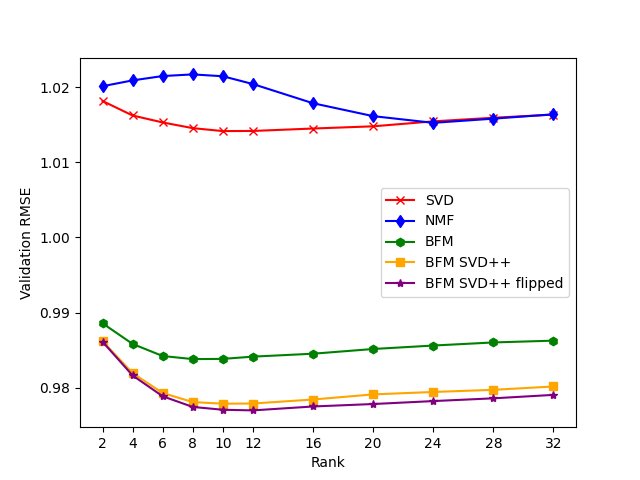
\includegraphics[width=\columnwidth]{figures/rank.png}
        \caption{Validation RMSE for different rank values.
        NMF performs best with a rank of 24 while others peak around 8 to 12.}
        \label{fig:rank}
    \end{figure}


    \section{Results}
    We present our results in \Cref{tab:ablation}, noting the Root Mean Squared Error \textbf{(RMSE)} of our baselines and final model.
    Test scores refer to the public leaderboard ranking on Kaggle obtained by training on the whole data while validation scores refer to a 10\% holdout of our training data.
    Models without test scores are added for the sake of completeness and not evaluated further as the performance was either not satisfactory or other models evaluated in the meantime performed better.
    Other models may only show test scores as they were directly evaluated on the test data to eliminate the need of
    fitting a second time.
    All scores are reported after clipping the outputs to~$[1, 5]$ unless stated otherwise.

    Our first baseline, SVD with rank 3, heavily depends on the initialization of unobserved values, achieving a test score of 0.9928 when replacing values with the item mean and only 1.0713 when using the overall mean.
    Due to this large discrepancy, we further experimented with more sophisticated initialization techniques such as using other models to predict unobserved values.
    In \Cref{tab:ablation}, \textit{10*SVD} stands for chaining SVD ten times one after another to iteratively predict unobserved values (leaving the observed values as is) for the input of the following.
    With this we were able to get a test score of 0.9882 which is a large improvement for SVD.
    Similarly, \textit{SVD + KernelNet} first trains the Kernel Net and then predicts the unobserved values such that they can be used to initialize the SVD which further decreased the test error to 0.9836.
    Chaining one SVD of rank 10 with our second best BFM model is able to reduce this further to 0.9710.
    Similar to the SVD, our second baseline, NMF, performs best when replacing missing values with the item mean and then chaining 10 NMF models which results in a validation score of 0.9946.
    In \Cref{fig:rank}, we varied the amount of singular values and reported the average performance of 3-fold cross validation.
    Here, we observed that except for NMF, which achieves the lowest error with rank 24, the other matrix factorization models perform best with a lower rank approximation of around 10.

    Next, we evaluate neural-based approaches.
    Starting with standard AE, we found that, when both the encoder and the decoder consist of a single hidden layer, increasing the width resulted in a better score.
    Furthermore, we have examined the effect of compositionality by using two layers which outperformed any single layer network, obtaining a validation score of 1.0539 after 250 epochs.
    NCF, our fourth baseline, already surpasses this performance only after 10 epochs and achieves its best score of 0.9787 after 250 epoch.
    Compared to that is the AutoRec which achieved an RMSE of 1.0100 after only 5 epochs after which the error steadily increased.
    Regarding the Kernel Net, replacing the unobserved values with zeros instead of item mean surprisingly fared best which is in contradiction to the insights gained from SVD, leading to a much better validation error of 0.9831 as opposed to 1.0409 after 150 epochs.
    From \Cref{fig:validation} it can be observed that overall the Kernel Net performed best, the AE made continuous progress, while AutoRec and NCF quickly started to overfit and diverge.

    \begin{figure}
        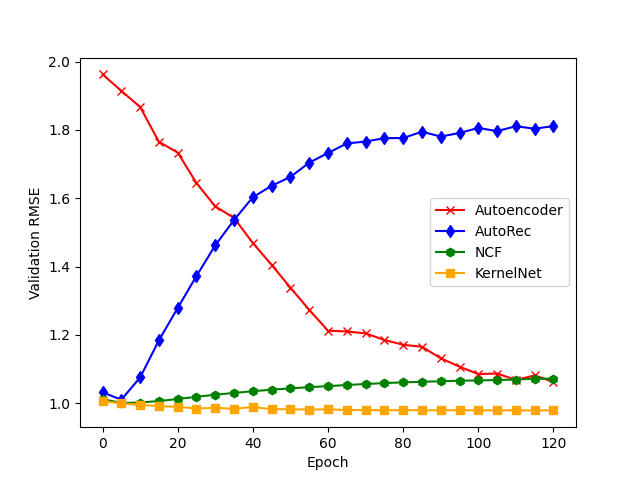
\includegraphics[width=\columnwidth]{figures/validation_plot.png}
        \caption{Validation RMSE for different epochs.
        AutoRec and NCF diverge after a few epochs while KernelNet and AE show the opposite behaviour.}
        \label{fig:validation}
    \end{figure}

    For BFM, we generally obtain similar results to~\cite{rendle_difficulty_2019}.
    As can be seen in \Cref{tab:ablation}, including both implicit features to BMF improves the score.
    Adding additional features for users and movies resulted in similar performance compared to the BFM SVD++ flipped model
    for almost all of our proposed features.
    Including distance metrics performed worse when compared to the genre clustering with size 18.

    Compared to that, the introduction of the Jaccard index performed similarly as well whereas the improved version of it surprisingly decreased the performance.
    As a final approach, we reformulated the problem of predicting user/movie ratings from a regression problem into a classification one (Ordered Probit) which yielded a slight performance gain, making it our best model with a final score of 0.9657.
    The heatmap of \Cref{fig:heatmap}, gives an overview on the conducted parameter search of sampling size per iteration and ranks for the BFM SVD++ flipped variant.

    \begin{figure}
        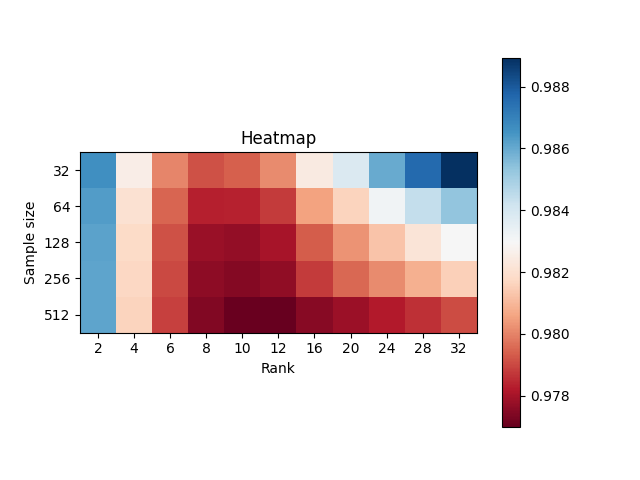
\includegraphics[width=\columnwidth]{figures/heatmap.png}
        \caption{Validation RMSE for different values of sample size and rank.
        We conduct the hyperparameter search on our second best model, BMF SVD++ flipped, due to the high computational burden of our best.
        Low-rank approximations of $8 - 12$ with high sampling sizes perform best.}
        \label{fig:heatmap}
    \end{figure}


    \section{Discussion}
    As stated in the previous section, the introduction of additional hand-crafted features for users and movies did not yield significant improvements for the BFM SVD++ flipped model.
    We assume that this is mainly based on the fact that the BFM model is already able to leverage this information and does not benefit from making this more accessible.
    Standard Jaccard index performed similarly, while genre clustering achieved exactly the same performance underlying the strong ability of BFMs to extract information from the data.
    However, other models may benefit from the improved accessibility, which we leave off for future work.
    Furthermore, the initialization of unobserved values is a key component as can be seen by the SVD results.
    Using the BFM SVD++ flipped model for initialization, we were able to achieve the best SVD test score.
    However, this still performs worse than the BFM on its own.
    Regarding our best model, users tend to overall rate movies rather positively than negatively for which we assume that this phenomenon can be better captured by formulating the problem of predicting user/movie ratings as a classification task (Ordered Probit).
    Moreover, when conducting the 3-fold cross validation, depicted in \Cref{fig:rank} and \Cref{fig:heatmap}, we observed that stratified sampling and shuffling is vital to the performance due to the nature of the dataset.
    For the heatmap, we further conclude that a low-rank approximations of around 10-12 in combination with a high sampling size is optimal for the BFM SVD++ flipped model.
    Surprisingly, this is different for our best model where a higher rank of 32 performed better.
    Lastly, using more sophisticated postprocessing techniques like rounding to integers or to quarters always resulted in worse performance.

    \section{Summary}

    In this paper we have examined the problem of collaborative filtering, analyzing a variety of models, such as SVD, NMF, NCF, Kernel Net, and AE networks.
    We explore variants of BFM, improving upon the score of the selected vanilla BFM baseline with implicit user/item features and reformulating the problem as a classification task instead of a regression one.
    Furthermore, we extend BFMs with additional features that represent movie genres as well as similarity measures between movies or users making this information more accessible and explicit for our model.

    \begin{table*}[h]
        \centering
        \begin{tabular}{|| c | c | c | c | c ||}
            \hline
            \textbf{Model}       & \textbf{Parameters}                       & \textbf{ Init Missing } & \textbf{RMSE}$_{test}$ & \textbf{RMSE}$_{valid}$ \\
            \hline
            SVD                  & Rank 3                                & total mean              & 1.0713                 &                         \\
            SVD                  & Rank 3                                & user mean               & 1.0558                 &                         \\
            SVD                  & Rank 3                                & item mean               & 1.0138                 &                         \\
            4*SVD                & Rank 3                                & item mean               & 0.9928                 & 0.9893                  \\
            7*SVD                & Rank 3                                & item mean               & 0.9894                 &                         \\
            10*SVD               & Rank 3                                & item mean               & 0.9882                 & 0.9854                  \\
            10*SVD               & Rank 3, Round Quarters                & item mean               & 0.9907                 &                         \\
            10*SVD               & Rank 10                               & item mean               & 0.9941                 &                         \\
            5*SVD + KernelNet    & Rank 3 | 150 Epochs                   & zero                    &                        & 0.9844                  \\
            5*SVD + KernelNet    & Rank 10 | 150 Epochs                  & zero                    &                        & 0.9838                  \\
            SVD + KernelNet      & Rank 10 | 150 Epochs                  & zero                    & 0.9836                 & 0.9803                  \\
            5*SVD + BFM SVD++ f. & Rank 3 | Rank 12                      & /                       & 0.9846                 &                         \\
            5*SVD + BFM SVD++ f. & Rank 10 | Rank 12                     & /                       & 0.9789                 &                         \\
            SVD + BFM SVD++ f.   & Rank 10 | Rank 12                     & /                       & 0.9710                 &                         \\
            \hline
            NMF                  & Rank 24                               & total mean              &                        & 1.0628                  \\
            NMF                  & Rank 24                               & user mean               &                        & 1.0497                  \\
            NMF                  & Rank 24                               & item mean               &                        & 1.0029                  \\
            10*NMF               & Rank 24                               & item mean               &                        & 0.9946                  \\
            \hline
            AE                   & 50 Epochs                             & total mean              &                        & 1.3382                  \\
            AE                   & 150 Epochs                            & total mean              &                        & 1.0757                  \\
            AE                   & 250 Epochs                            & total mean              &                        & 1.0539                  \\
            \hline
            NCF                  & 50 Epochs                             & /                       &                        & 1.0394                  \\
            NCF                  & 150 Epochs                            & /                       &                        & 1.0756                  \\
            NCF                  & 250 Epochs                            & /                       &                        & 1.0845                  \\
            \hline
            AutoRec              & 5 Epochs                              & zero                    &                        & 1.0100                  \\
            AutoRec              & 25 Epochs                             & zero                    &                        & 1.3723                  \\
            AutoRec              & 50 Epochs                             & zero                    &                        & 1.6625                  \\
            \hline
            KernelNet            & 50 Epochs                             & zero                    & 1.0003                 & 0.9939                  \\
            KernelNet            & 150 Epochs                            & zero                    & 0.9860                 & 0.9831                  \\
            KernelNet            & 150 Epochs                            & item mean               &                        & 1.0409                  \\
            KernelNet            & 450 Epochs                            & zero                    & 0.9886                 &                         \\
            \hline
            BFM                  & Rank 12                               & /                       &                        & 0.9727                  \\
            BFM SVD++            & Rank 12                               & /                       &                        & 0.9664                  \\
            BFM SVD++ f.         & Rank 12                               & /                       &                        & 0.9655                  \\
            BFM SVD++ f.         & Rank 32                               & /                       & 0.9688                 &                         \\
            BFM SVD++ f.         & Jacc. Sim., Rank 32                    & /                       & 0.9694                 &                         \\
            BFM SVD++ f.         & Improved Jacc. Sim., Rank 32          & /                       & 0.9974                 &                         \\
            BFM SVD++ f.         & Genre Clustering, Rank 32             & /                       & 0.9688                 &                         \\
            BFM SVD++ f.         & Mahalanobis Dist., Rank 32            & /                       & 1.0271                 &                         \\
            BFM SVD++ f.         & Euclidean Dist., Rank 32              & /                       & 0.9903                 &                         \\
            BFM SVD++ f.         & Ordered Prob., Rank 32                & /                       & \textbf{ 0.9657 }      &                         \\
            BFM SVD++ f.         & Ordered Prob., Round Quarter, Rank 32 & /                       & 0.9684                 &                         \\
            \hline
        \end{tabular}
        \caption{We note the Root Mean Squared Error (RMSE) on test and validation datasets to compare our baselines to our novelties.}
        \label{tab:ablation}
    \end{table*}

    \newpage

    \balance
    \bibliographystyle{IEEEtran}
    \bibliography{bibliography}
\end{document}
